%Incidencia de una onda plana a 45° con n_i = 1, n_t = 1.46   

\documentclass[tikz,crop]{standalone}

\usepackage{tikz}
\usetikzlibrary{decorations.pathreplacing,decorations.pathmorphing}
\usepackage{physics}

\begin{document}

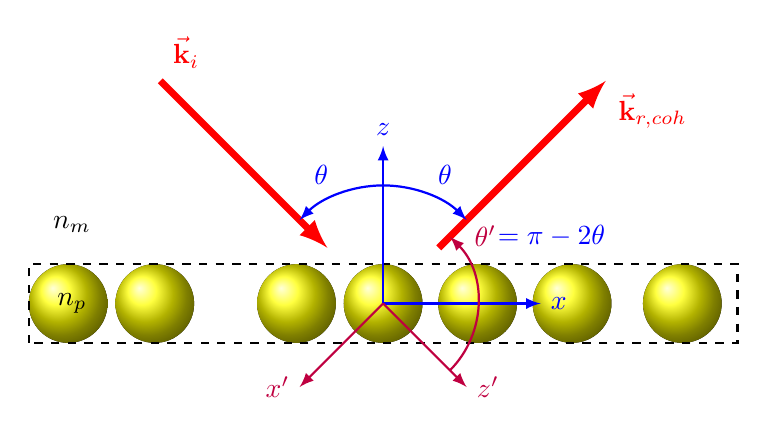
\begin{tikzpicture}[scale=1]
\def\a{.5}
\def\d{.5}

\foreach \x in {-4,-2.9,-1.1,0,1.2,2.4,3.8}{
\fill[ball color=yellow, opacity=1] (\x,0) circle(\a);}


\draw[thick, dashed] (-4.5,-\d) rectangle (4.5,\d);

\draw[latex -, thick, red, line width=2.5](135:1)--(135:4) node[anchor=south west]{$\va{k}_i$};
\draw[- latex, thick, red, line width=2.5](45:1)--(45:4)node[anchor=north west]{$\va{k}_{r,coh}$};

\draw[- latex, thick, blue] (0,0)--(90:2) node[anchor = south]{$z$};
\draw[- latex, thick, blue] (0,0)--(0:2) node[anchor = west]{$x$};
\path (0,0)++(135/2:1.5)node[anchor=south west, blue]{$\theta$}; 
\draw[- latex, thick, blue](90:1.5)arc(90:45:1.5);
\path (0,0)++(90+45/2:1.5)node[anchor=south east, blue]{$\theta$}; 
\draw[- latex, thick, blue](90:1.5)arc(90:135:1.5);

\draw[- latex, thick, purple] (0,0)--(-45:1.5) node[anchor = west]{$z'$};
\draw[- latex, thick, purple] (0,0)--(-135:1.5) node[anchor = east]{$x'$};
\path (0,0)++(30:1.2)node[anchor=south west, purple]{$\theta'$}; 
\path (0,0)++(30:1.2)node[anchor=south west, blue]{$\;\;\; =  \pi - 2\theta$}; 
\draw[- latex, thick, purple](-45:1.2)arc(-45:45:1.2);

\node at (-4,1) {$\; n_m$};
\node at (-4,0) {$\; n_p$};
\end{tikzpicture}
\end{document}
